\documentclass[a4paper]{article}

% ------------------------------------------------------------------------------
% Paquetes

% Input en Castellano
\usepackage[spanish]{babel}
\selectlanguage{spanish}
\usepackage[utf8]{inputenc}

% Pseudocodigo
% \usepackage[linesnumbered,lined,boxed,commentsnumbered,
% spanish,onelanguage]{algorithm2e}
\usepackage{algorithm}
\usepackage{algorithmic}

% Símbolos matematicos
\usepackage{amsfonts, amsmath, amssymb}

% Lemas, Teoremas
\newtheorem{teorema}{Teorema}
\newtheorem{lema}{Lema}
\newtheorem{prop}{Propiedad}

% Tablas
\usepackage{booktabs}
\usepackage[table,xcdraw]{xcolor}
\usepackage{multirow}

% Etc
\usepackage{indentfirst} % Sangría también en el primer parrafo
\usepackage[draft]{todonotes} % para poder tener notas con to-do's
\usepackage{capt-of} % Imágenes con captions.

% Simbolos Custom
% Cuando repetis mucho algo, ponelo acá

% Conjuntos
\newcommand{\Nat}[0]{\mathbb{N}} % Naturales
\newcommand{\Bin}[0]{\{0, 1\}} % Conjunto binario {0,1}

% Powerset, Conjunto de partes
\newcommand{\Pows}[1]{\mathcal{P}\left(#1\right)} % Powerset P(S)

% Complejidad
% See: https://texblog.org/2014/06/24/big-o-and-related-notations-in-latex/
\newcommand{\BigO}[1]{\mathcal{O}\left(#1\right)} %Big-O
\newcommand{\BigTheta}[1]{\Theta\left(#1\right)} % Complejidad Theta
\newcommand{\BigOmega}[1]{\Omega\left(#1\right)} % Complejidad Omega


% Links en los ítems del índice
\usepackage[colorlinks=true, linkcolor=black, citecolor=black]{hyperref}

% ------------------------------------------------------------------------------
% Caratula del DC


\usepackage{lib/caratula/caratula}
\materia{Algoritmos y Estructuras de Datos III}
\submateria{Primer Cuatrimestre de 2018}
\titulo{RTP 3}
\integrante{Alonso, Tomás}{396/16}{tomasalonso96@gmail.com}
\integrante{Bringas, Alejandra}{052/16}{abringas.t@gmail.com}
\integrante{Grosso, Alejandro}{016/16}{agrosso@dc.uba.ar}

% ------------------------------------------------------------------------------
\begin{document}

% Caratula
\maketitle

\tableofcontents
\newpage

% Secciones
\section{Introducción}

En este trabajo práctico se va a investigar y explorar la resolución de problemas con
diversas heurísticas de exploración de soluciones, en principal se va a trabajar
con búsqueda local, GRASP y algoritmos genéticos. Particularmente se va a intentar trabajar
con la toma de decisiones estratégicas en un juego de tipo adversarial.\\


En principio se pretende modelar un partido de fútbol donde dos equipos de 3
jugadores compiten para ver cuál de los dos obtiene más goles en un período de tiempo. El
equipo con mayor cantidad de goles será el ganador. En caso de que ambos equipos tengan
la misma cantidad de goles realizados, el resultado será un empate. Nuestro objetivo es lograr
conseguir un equipo que tenga una buena estrategia de juego con las mencionadas técnicas
algorítmicas. El objetivo es, en primer lugar, modelar computacionalmente el fenómeno descrito, luego
parametrizar propiedades de dicho modelo que sean controlables e implementar, con distintas técnicas
algorítmicas, algoritmos que permitan conseguir buenos valores para dichos parámetros. Estos parámetros
serán los generadores de distintas soluciones al problema modelado.
\\


Se procederá así:
En la próxima sección se describirá el modelo lógico y luego, con más detalle, cómo fue implementado
computacionalmente el mismo,
así como también una explicación de cada decisión tomada ya sea por necesidad o facilidad para
la aplicación de las heurísticas sobre esta implementación. El objetivo es que una solución
para el modelo sea también una solución para el problema real.
\\


Luego se explicará el razonamiento y las decisiones tomadas en cuanto a las ideas desarrolladas para
la resolución del problema. Se mostrara cómo funciona la heurística tratada en particular,
daremos también ejemplos del funcionamiento y se explicará en detalle por qué es
efectivamente una implementación de la técnica elegida, hablaremos también de qué esperamos notar
en los resultados y de la complejidad temporal de cada algoritmo.
\\


Por último vamos a realizar una experimentación computacional para medir la performance de
los algoritmos implementados así como sus distintas propiedades. Para ello vamos a trabajar con
todas las heurísticas al mismo tiempo, comparando sus resultados para corridas del aproximadamente
el mismo costo temporal. Luego se van a desarrollar experimentos que permiten medir los aspectos
evolutivos de las soluciones obtenidas mediante las distintas técnicas utilizadas en
el trabajo para poder compararlas entre sí en base a estos aspectos.\\


\newpage
\section{Modelado}

El Juego básicamente consiste en un tablero rectangular de $n \times m$ donde
$n$ es $2m$ y $m$ es impar, con un arco de tres posiciones, compiten dos equipos
de tres jugadores un partido de fútbol con un numero de jugadas determinado.


El objetivo principal es desarrollar un equipo que con una función parametrizable
que evalúa posibles jugadas siguientes y con eso decida cual es la mejor a tomar
la idea es, con las distintas heurísticas, decidir que parámetros son buenos para esa
función evaluadora y así diagramar una buena estrategia de juego general.\\

\subsection{Implementación}


Para implementar el juego se decidió utilizar todas estructuras de diseño propio así poder
detectar de mejor forma cualquier error que ocurriese, lo cual no fue el caso al intentar
usar lo proveído por la cátedra.
En primer lugar se decidió hacer un tablero, el mismo es el que tiene las dimensiones de la cancha y
conoce todas las reglas del juego a ser respetadas por los equipos, también tiene consigo la pelota y los
6 jugadores, el es el encargado de llevar la partida y el resultado así como también es el que tiene la
función evaluadora de jugadas que toma los genomas (los parámetros de la función dependientes de cada equipo)
y evalúa la jugada a realizar.
Luego esta el equipo, que solo tiene identificadores para sus jugadores y el dicho genoma propio de cada equipo.\\


Todas las estructuras que manejan una posición (jugadores y pelota) tienen en realidad, dos posiciones, actual, la que
tiene actualmente luego de la ultima jugada, y también siguiente, la posición que, de acuerdo al
movimiento elegido para evaluar, el tablero utiliza para poner la posición que va tener en la próxima jugada y así
saber como quedaría configurado el terreno para evaluarlo
El tablero usa esta variable siguiente para evaluar el puntaje de la jugada a tomar.
luego el tablero le dice los puntajes de las jugadas propuestas al equipo y este decide cual realizar, confirmandole
al tablero cual es, y este efectivamente realizando la jugada, que es básicamente actualizar la posición actual
con la siguiente.\\

\subsection{Parametrización}

Se decidió utilizar un genoma de 30 parámetros los cuales varían entre $-1$ y $1$ simbolizando la importancia total
que se le da a un dato del tablero ($-1$ si es muy malo que eso crezca $0$ si es irrelevante $1$ si es muy bueno que crezca)
y también se utilizan algunos para cuando se tiene la pelota y otros distintos para los mismos datos
cuando no se posee la pelota. El motivo de esto es poder permitirle a los equipos tomar estrategias distintas cuando están
atacando o defendiendieno, se presento la idea de también permitir actuar distinto cuando se va perdiendo o ganando pero
el tiempo no permitió implementar esto y ademas creemos que ya vamos a poder ver un buen comportamiento con solo esta
diferenciacion.\\

Los últimos 3 genes del genoma no varían entre $-1$ y $1$, solo van de $0$ a $1$ y representan las probabilidades de quite
de los 3 jugadores del equipo, supusimos que esto es importante para el juego y decidimos darle el poder de esto
a los algoritmos de optimizacion.\\


El tablero simplemente toma este genoma y dependiendo si el equipo esta en poseción o no, multiplica el valor del gen por
el dato siendo considerado, como por ejemplo puede ser la distancia de un jugador al arco, al rival, la distancia de la pelota
al arco contrario, la distancia a los borde, el área cubierta y si el siguiente paso es gol o no.


\newpage
\section{Optimización de parámetros}
Buscar jugadas es $\BigO{1}$ debido a que la cantidad de movimientos que puede
hacer cada jugador es acotada, luego las combinaciones de movimientos posibles
son acotadas. Como mover jugadores en el tablero, en el peor caso, significa
mover todos los jugadores, más la pelota y los cálculos de disputa y de gol son
constantes, mover tablero es constante. Luego, cada paso del juego es constante.
Entonces, la complejidad de un partido varía en base al tiempo de juego, dando
una complejidad de $\BigO{\textrm{tiempo de juego}}$, a lo largo del tp
llamaremos $t$ al tiempo de juego.

\subsection{Grid-Search:}

La lógica de grid-search es plantear todo el espacio de soluciones posibles,
como este espacio es muy extenso, que en este trabajo corresponde a todos los
valores continuos de -1 a 1 que puede adoptar cada uno de los 30 genomas, no es
computacionalmente posible recorrer todo, por eso se decide empezar en algún
punto aleatorio y, con un criterio, recorrer todas las soluciones vecinas a esta
para tomar la mejor. Repitiendo el proceso hasta llegar a alguna que sea mejor que
todos sus vecinos, a este procedimiento se lo llama búsqueda local.


\subsubsection{Búsqueda Local:}


Nuestro espacio de soluciones son todas las combinaciones posibles de genes
distintos en un genoma, son 30 genes que van en los reales entre $-1$ y $1$,
entonces se comienza con un equipo aleatorio, es decir, con un genoma aleatorio,
luego se define la vecindad como todos los genomas que tiene un solo gen
cambiado en $\pm 0.1$ y saturando si llega a $-1$ o $1$ o a $0$ o $1$ en caso de
tratarse de una probabilidad. Con estos genomas se lo hace jugar secuencialmente
quedándose con el ganador siempre y, finalmente con el último ganador. Como
criterio para finalizar la búsqueda, se itera hasta que un genoma sea
mejor que todos sus vecinos, es decir, gane a todos sus vecinos.

\paragraph{Complejidad:} Debido a que el espacio de soluciones se discretizó, la
cantidad de soluciones es acotada, en particular es de 21 posibilidades por cada
genoma y 11 posibilidades para las probabilidades, lo que da un número de
$21^{27}+11^3$. Como en el peor caso se recorrería todo el espacio de busqueda,
la complejidad es $\BigO{\textrm{t}}$.

\subsubsection{GRASP:}


La lógica de GRASP es simplemente tener muchas soluciones aleatorias con
búsqueda local, es decir, máximos locales y luego, con todos estos mejores de
sus vecinos, se realiza un torneo para obtener el mejor de todos esos . El
concepto se basa en que con la búsqueda local lo más probable es solo obtener un
máximo local y no el mejor de todos, entonces con GRASP la idea es aumentar la
probabilidad de obtener el mejor global o al menos obtener un buen máximo local.

El algoritmo está implementado como un ciclo de búsquedas locales.

Creemos que GRASP va a dar resultados útiles en pocas iteracions, pero que va a
ser mucho mas costoso obtener resultados mejores y realmente buenos en
comparación con los que pueda obetener el genético con el mismo tiempo de
ejecución.

\paragraph{Complejidad:} Cada búsqueda local tiene complejidad $\BigO{t}$, luego
se realizan $k$ búsquedas locales, donde $k$ es la cantidad de iteraciones de
GRASP, dando una complejidad de $\BigO{t\times k}$. Por último, se realiza un
torneo entre todos los máximos locales, siendo la complejidad la de {\it
  fitness\_puntos} (ver complejidad en genético), dando por resultado una
complejidad de $\BigO{t\times k + k^2\times t} = \BigO{k^2\times t}$.

\subsection{Algoritmos genéticos: breve contexto}

Para la siguiente sección leímos tres publicaciones académicas que utilizan el esquema de algoritmos genéticos para optimizar parámetros relacionados con los modelados de los distintos problemas que presentan. Se aplican sobre, por ejemplo, planeamiento de almacenamientos logísticos\cite{warehouse}, agentes que aprenden a jugar al Mario\cite{mario} y modelos epidémicos que pretenden detener la proliferación de enfermedades\cite{epidemic}. Mientras leíamos estas publicaciones (y mientras decidíamos cuáles leer entre un mar de títulos interesantes) comprendimos que los algoritmos genéticos son aplicables a variadas ramas del conocimiento. Entendimos también que los resultados obtenidos dependen fuertemente de buenas decisiones a la hora de instanciar todas las partes de este esquema. Resulta imprescindible determinar una función de \emph{fitness} adecuada, que contemple las variables necesarias y ajustarla a medida que se conozcan los primeros resultados de la experimentación hasta obtener una que permita lograr buenos resultados.


\subsubsection*{Playing Mario using advanced AI techniques:}

Con un algoritmo genético buscaron optimizar los pesos de una red neuronal (es como si fuera una calibración) que decide las
jugadas basándose en el estado del entorno de Mario. Las salidas de esta red representan las cinco posibles teclas que pueden
usarse para la siguiente jugada.
Este estado de entorno tiene 14 parámetros, que dan información sobre la poscición de los obstáculos/enemigos.


En el paper se discuten distintos parámetros a tomar en cuenta para la función de \emph{fitness} y ciertos obstáculos como
la generalización del entrenamiento a más niveles del juego, pues las poblaciones del algoritmo genético iban olvidando cómo
 evitar enemigos anteriores una vez que llegaban a niveles más avanzados.

\subsubsection*{A Genetic Algorithm for Finding an Optimal Curing Strategy for Epidemic Spreading in Weighted Networks:}

Esta publicación presenta el problema de evitar la expansión de una epidema buscando el menor costo. Se basa en modelos
 epidémicos modelados sobre grafos pesados, que además del uso medicinal tienen aplicaciones en redes sociales y
 telecomunicaciones. Por ejemplo, una epidemia en una red social podría se la difusión de una noticia falsa.


El modelo asume que un nodo puede infectarse varias veces luego de recuperarse y por teoremas previos se cuenta con
que existe un valor umbral tal que si se pasa, la epidemia quedará siempre en la red. Es decir, cada nodo va a infectar
 a otro y cuando se recuperen van a volver infectarse indefinidamente. Este umbral se traduce en una propiedad que
 deben cumplir los parámetros que más adelante se explican.
Los nodos tienen una tasa o velocidad de recuperación luego de una infección, que puede ser modificada, por ejemplo,
distribuyendo más vacunas a la ciudad representada por ese nodo. Tienen además un costo asociado, que puede ser el costo
 de distribución o de la cantidad de vacunas necesarias. Lo que se busca entonces es un conjunto de tasas de recuperación,
 una para cada nodo, tal que cumplan la propiedad relacionada al umbral epidémico y a la vez minimicen el costo.


Se utiliza un algoritmo genético para encontrar un buen valor para estas tasas. Muchas de las partes, como la función de
cruzamiento, fueron utilizadas desde la herramienta MATLAB.
Los resultados, evaluados sobre redes reales y sintéticas, se compararon con la herramienta actual utilizada para este
tipo de problemas. Se muestran en casi todos los casos costos mucho menores obtenidos con el algoritmo genético.

\subsubsection*{Multi-Objective Genetic Algorithms / Multi-Objective Optimization:}

Como comentario final, se pudo observar una gran cantidad de papers que trataban sobre algoritmos de este estilo, genéticos
multi-objetivo, la lectura de los mismos se torno ardua ya que se manejaban términos muy específicos y técnicos no vistos
en las clases. Pero en lineas generales y buscando informacion\cite{MOO} sobre este tema en particular se pudo entender
que, muy básicamente, se tratan de algoritmos que trabajaban maximizando varias funciones en paralelo, en particular
para los algoritmos geneticos se trata de las funciones de \emph{fitness}, las cuales quizás no resultan siempre
directamente compatibles, o hasta contradictorias, entonces se entra en un juego de comprometer alguna
para mejorar otra y se acomplejiza el procedimiento de mejora, pero el concepto evolutivo general, es sin dudas, el mismo.

\subsection{Implementación del Algoritmo Genético:}

La idea del algoritmo genético se basa en la teoría de la evolución, consiste en generar una población,
en principio aleatoria, de muchos genomas, con estos se testea cuan buena solución son para el problema dado.
En este caso, como se trata de un juego, se prueba en un torneo con una función puntuadora
(\emph{Fitness}) cuales ganan mas partidos o juegan mejor, luego, en base a esto se eligen cuales van a permanecer
cuales van a reproducirse y cuales desaparecen \emph{Selección} y con los que tienen descendencia se utilizan
las funciones de \emph{Crossover} y de \emph{Mutación}.

De todo esto se va a hablar en las próximas partes:

\subsubsection{Fitness:}


La primera, \emph{fitness\_puntos} , se basa en la idea de un torneo de fútbol del mundo real, simplemente hace jugar a todos
los equipos entre si (como en una liga) y les suma $3$ puntos por ganar, $1$ por el empate y $0$ por perder.
Esperamos que esto presente un buen método de evaluación ya que se basa en algo real, y es simple en cuanto a que solo importa ganar
mas partidos, lo cual, a fin de cuentas, es lo mas importante.\\

La segunda función, \emph{fitness\_diff\_goles} trabaja de la siguiente forma, si gana le suma un punto y luego le suma tantos
puntos como diferencia de gol tenga con el contrario, por ejemplo, si gano $3$ a $1$, le suma $2$ puntos mas al obtenido por
la victoria.

Esta función intenta reforzar a los equipos que hagan muchos goles, lo cual podría llegar a indicar que juegan mucho mejor que el
contrario y podría significar que va a jugar mejor también contra otros potenciales adversarios.\\

Al final de la ejecución, ambas funciones ordenan la población de acuerdo a los puntajes para facilitar el trabajo de las funciones
de selección


\subsubsection{Selección:}


\subsubsection{Crossover:}


\subsubsection{Mutaciones:}


\todo[inline]{alguna conclusion previa sobre lo que creiamos que iba a pasar}


\newpage
\section{Experimentación}
% Para cada generación tomamos la media y la varianza de los puntajes de todos los individuos. Creemos que es bueno tener un genoma que provenga de una generación cuya varianza sea baja, ya que esto significaría que los

A lo largo de toda la experimentación nos encontramos con el problema de que los resultados de los partidos llegaban a depender
fuertemente del lado que tenia cada equipo, no pudimos concluir por que sucedía esto exactamente y no disponemos del tiempo
para revisar en profundidad el código, creemos que el error yace en el tablero en si (como implementamos las reglas del juego),
 o en la función evaluadora de jugadas la cual puntúa distinto según el lado, lo cual no debería suceder.
 esto fue tomado en cada una de las secciones siguientes para poder sortear los problemas que nos traía de la mejor forma posible.


A parte de esto, se ecuentran por lo general buenos comportamientos de juego de algunos equipos.

\subsection{Genético}


Iniciamos nuestra experimentación con el algoritmo genético.
Tuvimos grandes complicaciones para experimentar con las distintas funciones de selección y crossover implementadas, pues constantemente encontramos errores o comportamientos no deseados en los partidos.
Por ejemplo, nos dimos cuenta de que se llegaba a un momento en que los jugadores maximizaban el aŕea ocupada por su equipo y estaban muy cerca del rival, pero la pelota se encontraba sola y nadie iba a buscarla.
Agregamos entonces el genoma que relaciona a los jugadores con su distancia a la pelota, para que tuvieran una mejor visión del campo de juego, y quitamos el que mide el área cubierta por los jugadores de un mismo equipo.
No se presenta en detalle en este informe, pero se observan mejoras respecto a esa situación: los jugadores ya no se quedan trabados, sino que en casi todo momento alguno tiene la pelota.

Una gran barrera también fue el tiempo, pues aumenta muy rápidamente al agrandar las poblaciones.
Consideramos entonces una población de 15 individuos y 30 generaciones. A esto se le agregan los parámetros 0,2 y 0,4 como fracción de selección y probabilidad de mutación respectivamente (explicadas en la Sección \ref{genetico-seleccion}).
En cuanto a parámetros del juego en sí, tenemos un tablero de $5\times10$ y tiempo 70.
Fijamos las posiciones iniciales de los jugadores de manera simétrica, intentando tener la menor cantidad de diferencias entre los que comiencen de un lado y de otro.
Dada la cantidad de funciones distintas que implementamos para un mismo fin, como dos de selección de individuos, dos de crossover de genomas y dos de mutaciones, realizar todas las posibles combinaciones fue temporalmente inviable. Siguiendo el espíritu futbolísitico del trabajo, decidimos diagramar un pequeño ``torneo'' de funciones. En el mismo pensamos comparar cada tipo de función, partiendo de una combinación arbitraria, y observar el partido entre los equipos resultantes. El equipo ganador determinará qué función se utilizará en la siguiente instancia. Los genomas resultantes pueden verse y probarse en el archivo \texttt{tp3.cpp}.



% \todo[inline]{VER POR QUÉ CAMBIA EL RESULTADO DE LOS PARTIDOS DEPENDIENDO DEL LADO EN QUE EMPIECEN}

\subsubsection*{Crossover: Bloques vs. Aleatorio (6 (Izq) - 4(Der))}

\textbf{Funciones usadas: } fitness$\_$puntos, seleccion$\_$por$\_$cantidad, mutacion$\_$A.


% Genoma bloque:-0.775167, -0.268792, -0.904803, 0.509839, 0.0429661, -0.749711, -0.330696, -0.72851, 0.402388, -0.690626, -0.925932, -0.548266, -0.311845, 0.474691, 0.0257145, 0.784108, -0.86784, -0.262816, 0.852761, -0.65904, 0.515403, 0.490343, 0.458956, -0.679425, -0.982449, -0.845339, 0.519684, 0.749116, 0.0456578, 0.550204, 0.0943544

% Genoma random: -0.709169, 0.36851, -0.520018, 0.6342, -0.0282138, 0.322789, -0.616418, -0.854534, -0.545993, 0.164261, 0.16543, 0.492899, -0.592142, -0.209919, -0.923623, 0.584831, 0.381569, -0.133004, -0.995532, -0.254421, 0.639068, 0.0105143, 0.494118, -0.125545, -0.821469, -0.731869, 0.141382, 0.793763, 0.388867, 0.428832, 0.170146

Los equipos no tienen mucho problema para anotar goles, aunque sí para robar la pelota.
Si bien ambos tienen un jugador que se queda en una esquina parado, en cada oportunidad que un equipo tiene la pelota logra meter un gol, con algún oponente marcando de cerca.
Sucede dos veces que el equipo izquierdo (el generado por crossover en bloques) logra robar la pelota y arruinar los planes de gol del equipo contrario. De esta manera logra sacar dos puntos de diferencia.


\subsubsection*{Fitness: Puntos (torneo) vs. Diferencia de goles (4 (Izq) - 2(Der))}

\textbf{Funciones usadas: } seleccion$\_$por$\_$cantidad, crossover$\_$BLOQUES, mutacion$\_$A.

% Genoma puntaje: -0.0912428, 0.441283, 0.526057, -0.24552, -0.495963, -0.44873, -0.994717, -0.158943, 0.652438, 0.664869, 0.230037, 0.374349, -0.995683, 0.800342, -0.515715, 0.741213, 0.356681, 0.0936855, -0.615283, -0.43112, 0.101387, 0.222677, -0.500011, 0.0475549, -0.874837, 0.190928, -0.818234, 0.50323, 0.514024, 0.230156

% Genoma dif_goles: 0.0354922, -0.347757, -0.00128968, -0.454219, -0.352621, -0.698883, -0.959573, -0.730346, -0.451026, -0.855564, -0.898217, 0.594382, -0.377874, -0.126251, -0.297974, 0.196175, 0.964436, -0.592206, -0.578612, 0.277421, -0.015946, -0.471911, -0.019213, -0.182925, -0.847654, -0.218569, 0.730436, 0.622654, 0.912127, 0.818418

A diferencia del partido anterior, se observan muchas jugadas frustradas por quites.
Se ve también que el jugador que tiene la pelota siempre está marcado por un oponente, lo cual está íntimamente relacionado con la gran cantidad de quites ocurridos.
Fue un partido muy emocionante, ya que además hubo pases.
Una estrategia muy repetida del equipo izquierdo (el generado con fitness$\_$puntos) fue sacarle la pelota al oponente bien cerca de su propio arco y hacer un pase a un jugador que estaba cerca.
El mismo se encargaba luego de llevar la pelota hasta la otra punta de la cancha y meter gol.\\

Observamos que los equipos y sus jugadas van mejorando a medida que avanza este torneo: más quites, pases entre jugadores, algunos que marcan y en este partido no hubo jugadores que se quedaran quietos o que alternaran entre dos posiciones contiguas.
Por esto creemos que lograremos un equipo relativamente bueno para el final de las comparaciones.


\subsubsection*{Selección: Cantidad vs. Puntaje (4 (Izq) - 3(Der))}
\textbf{Funciones usadas: } fitness$\_$puntos, crossover$\_$BLOQUES, mutacion$\_$A,.

En este partido se ven muchos quites también, pero resalta en ambos equipos que las jugadas son llevadas a cabo por un único jugador.
Los demás raramente se mueven, aunque uno de los del equipo izquierdo estuvo donde tenía que estar para quitar la pelota al oponente, evitar un gol y pasársela a su compañero goleador.

Nos gustaría decir que seleccionando los individuos por una cantidad fija se logra mayor estabilidad en la estrategia de juego, pero ambos equipos tienen un comportamiento muy parecido: un único jugador muy activo que se encarga de anotar goles, quitar la pelota y marcar al oponente. Atribuimos la victoria del equipo izquierdo en gran parte al azar, pero esto es suficiente para que la combinación de funciones utilizadas para generarlo pasen a la siguiente instancia.

\subsubsection*{Mutación: Aleatorio vs. Valor opuesto (1 - 1)}
\textbf{Funciones usadas: } fitness$\_$puntos, seleccion$\_$por$\_$cantidad, crossover$\_$BLOQUES.

De manera parecida al partido anterior, se observan un jugador protagonista de cada equipo. Los demás jamás tocan la pelota y se mantienen casi siempre en el mismo lugar. Quienes sí manejan la pelota se mueven casi siempre en el mismo casillero, constantemente disputando la pelota. Hay muchos quites, idas y vueltas. Es tal la situación que en los mismos 70 tiempos en los que en otros partidos se anotaron 10 goles, en este se anotaron solamente 2, uno para cada equipo. Sucedió algo llamativo, que fue que uno de los jugadores se quedó parado con la pelota al lado de su arco hasta que el opontente se la quitó y anotó un gol.

Además de probar algunas instancias de las distintas partes del esquema de algoritmo genético pudimos ver que existieron variadas estrategias que igualmente ganaron. Cada una de ellas se relaciona a un genoma, para el cual no vimos convergencias claras. Sí pudimos observar que ciertas coordenadas tomaron siempre valores negativos, como por ejemplo la distancia de los primeros jugadores al arco cuando tienen la pelota. Como se explica en la sección de parametrización, esto significa que el equipo va a elegir las jugadas que minimicen esa distancia. No es casualidad que en todos los genomas obtenidos estos valores hayan sucedido para los jugadores número 0 y que los demás tengan valores positivos para la misma distancia en casi todos los genomas, ya que esos jugadores con valores positivos eran quienes no participaban tanto en la ejecución de los goles.

Esta curiosidad de los valores se repitió para el gen 13, que se relaciona con la distancia del rival cuando no se tiene la pelota. Esto tiene sentido, pues cuando no se tiene la pelota es conveniente acercarse al oponente. En siete de los ocho genomas este valor fue negativo y en cinco el valor estuvo entre -0.995683 y -0.829386. Podríamos esperar que con más generaciones este gen efectivamente converja a un valor similar.



\subsection{Grid-Search}

La experimentación con \emph{Grid-Search} se basó en usar \emph{GRASP} ya que \emph{búsqueda local} es solo un caso particular
de correr \emph{GRASP} en una sola iteracion.
Primero se corrieron experimentos cortos para probar la efectividad del algoritmo y se obtuvieron equipos relativamente buenos,
a pesar de algunas problemáticas presentadas por el juego y la función evaluadora ademas de los genomas en principio defectuosos,
estos jugaban y metian goles.\\

Luego, cuando se llego a una versión final del juego, nos encontramos con que el algoritmo, al generar los vecinos, nos generaba también
el vecino anterior del que venia, esto junto con que también descubrimos que el resultado de los partidos dependía del lado en el
que se jugaba, causo lo que seguro iba a pasar, el algoritmo se quedaba saltando entre $2$ vecinos que se ganaban mutuamente y no
salia de ese ciclo.
Para evitar esto se decidió no generar el vecino del que se venia. Esta solución es parcial y no es la mejor, pero como se dijo primero,
no encontramos el error original y esta solución nos permitió seguir avanzando con el proceso de \emph{GRASP}.\\


La experimentación de este procedimiento no es muy variada ya que solo consiste en dar una cantidad de iteraciones y dejar que
busque localmente varios resultados para luego hacerlos competir, se puede decir que el tiempo que tarda en encontrar
cada resultado es corto, no pasa por lo general de entre $1$ minuto y $5$ minutos y como máximo ha llegado a tardar $10$ minutos, sin tener en cuenta
los diversos casos en los que no terminaba.


Se corrió un grasp de 50 iteraciones con la ultima versión y el genoma encontrado es el utilizada para competir contra el mejor que se logro encontrar
corriendo el genético. No se encuentra mucha mas experimentación que esta ya que el concepto bajo el que trabaja \emph{GRASP}
es simple y no presenta muchas posibilidades de variación en su idea para compararlas, lo primero que se ocurre para realizar
experimentación es un cambio en la vecindad utilizada para buscar localmente pero no hemos logrado diseñarla por cuestiones
de tiempo y priorizacion del método genético, sin embargo
creemos que la propuesta es una buena decisión que ademas fue discutida con un profesor.


\newpage
\section{Conclusión}
En este trabajo propusimos un modelado del juego planteado en el enunciado y dos heurísticas para optimizar sus parámetros.
El modelado nos tomó mucho tiempo por su complejidad.
Hubiéramos preferido dedicarle más tiempo a realizar distintas funciones de fitness, por ejemplo, pero el hecho de encontrar errores en el juego nos hizo volver una y otra vez al código base.

A pesar de no haber conseguido equipos que jueguen de manera profesional, consideramos un gran logro el hecho de que haya marcas, quites, pases y goles.
Viendo los partidos y los comportamientos de los equipos, es evidente el potencial de los métodos para obtener buenos parámetros en los genomas.
Como nuestro juego presenta algunos problemas, la comparación entre dos equipos no es fácil y no creemos que el resultado refleje con exactitud las diferencias. Pero las comparaciones de las distintas funciones utilizadas en el algoritmo genético sí dan resultados y comportamientos interesantes de analizar.
Igualmente encontramos ciertas tendencias en algunos de los genes que se corresonden con cierta manera de jugar.
Nos hubiera gustado experimentar con poblaciones más grandes y más generaciones, que tal vez hubieran logrado un resultado mejor.

Nos quedó pendiente encontrar la razón detrás de la diferencia de jugadas si se empieza de un lado u otro.















 % En principio se debe decir que se cumplieron, en mayor o menor medida, todos los objetivos
 % propuestos por el enunciado y por el grupo, quizás no logramos pulir todos los aspectos
 % necesarios para poder llegar a una etapa de experimentación "limpia", igualmente llegamos
 % a datos coherentes.

 % Es importante decir que se explica con correctitud las decisiones tomadas y el resultado final
 % de la implementacion general del trabajo, desde las estructuras usadas hasta las ideas que
 % definieron como se decidió utilizar las heurísticas.

 % En base a todo esto, podemos decir que hubiésemos preferido orientar el trabajo más a
 % las heurísticas que a las partes necesarias para que estas puedan trabajar, pero por diversas
 % cuestiones encontramos mayores dificultades con esto y no fue posible.

 % El partido final entre ambas heurísticas resultó en una victoria para

 % ...

 % pero,
 %  como nuestro juego presenta algunos problemas, la comparación entre ambos no es fácil
 %  y no creemos que el resultado refleje con exactitud las diferencias. Pero las comparaciones
 %  de las distintas funciones utilizadas en el algoritmo genético si dan resultados y comportamientos
 %  muy interesantes de analizar.


\newpage
\section{Referencias}

\begin{thebibliography}{9}
\addcontentsline{toc}{section}{References}
\bibitem{warehouse}
C. Pan, S. Yu, X. Du.
\textit{Optimization of Warehouse Layout Based on Genetic Algorithm and Simulation Technique.}
Dalian Neusoft University of Information, China. 2018.

\bibitem{mario}
L. D. Jørgensen, T. W. Sandberg.
\textit{Playing Mario using advanced AI techniques.}
2009

\bibitem{epidemic}
C. Pizzuti, A. Socievole.
\textit{A Genetic Algorithm for Finding an Optimal Curing Strategy for Epidemic Spreading in Weighted Networks.}
Inst. for High Perform. Comp. and Networking (ICAR), National Research Council of Italy (CNR). Presentado en GECCO ’18.

\bibitem{MOO}
\textit{Multi-objective optimization.}
Articulo de wikipedia en el cual se obtuvo la informacion basica de optimizacion multi-objetivo.\\
\url{https://en.wikipedia.org/wiki/Multi-objective_optimization}

\end{thebibliography}


\newpage
\section{Anexo}\label{ANEXO}

{\centering
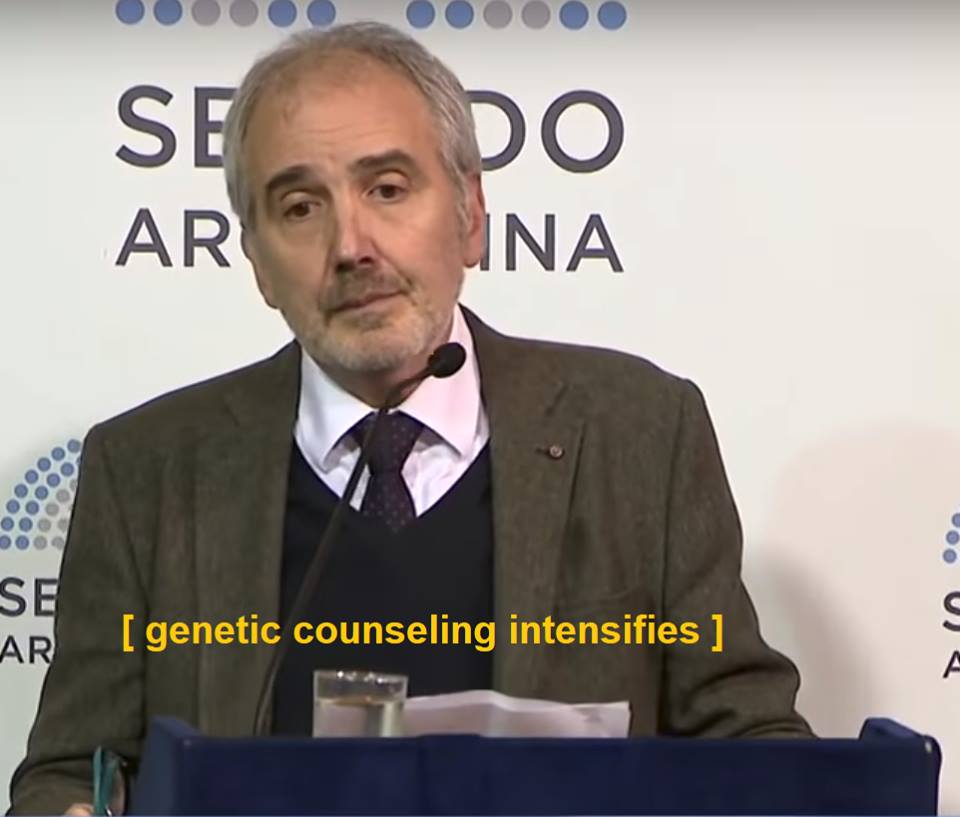
\includegraphics[width=1\textwidth]{kornblicounseling.jpg}
}
\end{document}
